%!TEX root = ../StatisticalCorrelations.tex

\graphicspath{{Body/Figures/EvW/}{Body/Figures/GoodnessOfFit/}{Body/Figures/Correlations/}}

\section{Monte Carlo Details}


In order to determine the correlation coefficients between the various analyses, a Monte Carlo simulation was developed which includes information from real data and incorporates the various analyzer parameters as given in \tabref{tab:analyzerParameters}. This Monte Carlo generated pseudo-data according to the different analysis types, reconstructions, and datasets, filled histograms defined by the various parameters, and then fit the resulting samples. The fit parameters from the samples were then plotted against one another and the correlation coefficients calculated for the different datasets.


\subsection{Generating Function}

Pseudo-data was generated using \ROOT's \texttt{TF2->GetRandom2()} method. The 2D function used to generate the data is given by a five parameter function with energy dependence on the number, asymmetry, and phase terms,
\begin{align}
    N(t, E) = N_{0}(E) \cdot e^{-t/\tau_{\mu}} \cdot (1 + A(E) \cos{(\omega_{a}t + \phi(E))}),
\label{eq:2dfunc}
\end{align}
with the time-dilated muon lifetime \taumu equal to \ns{64440} and the \gmtwo frequency \wa set as in \equref{eq:wa}, with \R set to 0. 


\begin{figure}
\centering
    \begin{subfigure}[t]{0.45\textwidth}
        \centering
        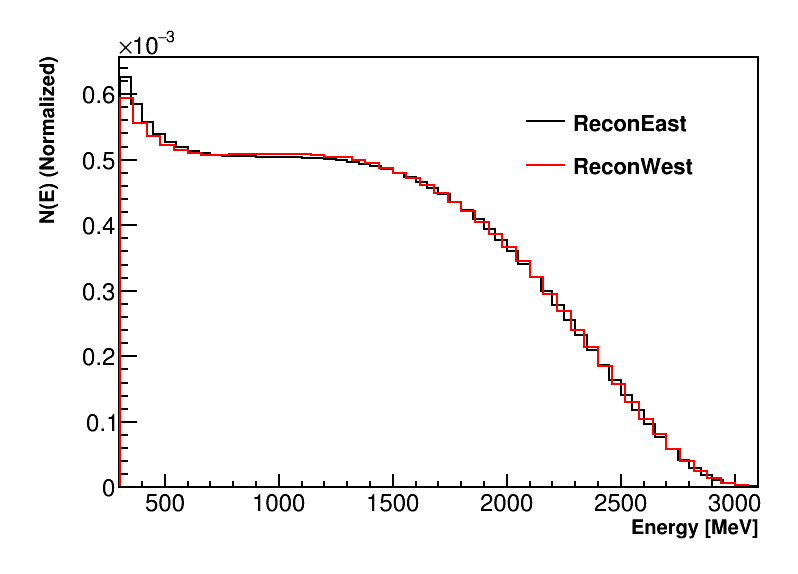
\includegraphics[width=\textwidth]{ReconEastvWest_N}
        \caption{$N(E)$}
    \end{subfigure}% %you need this % here to add spacing between subfigures

    \begin{subfigure}[t]{0.45\textwidth}
        \centering
        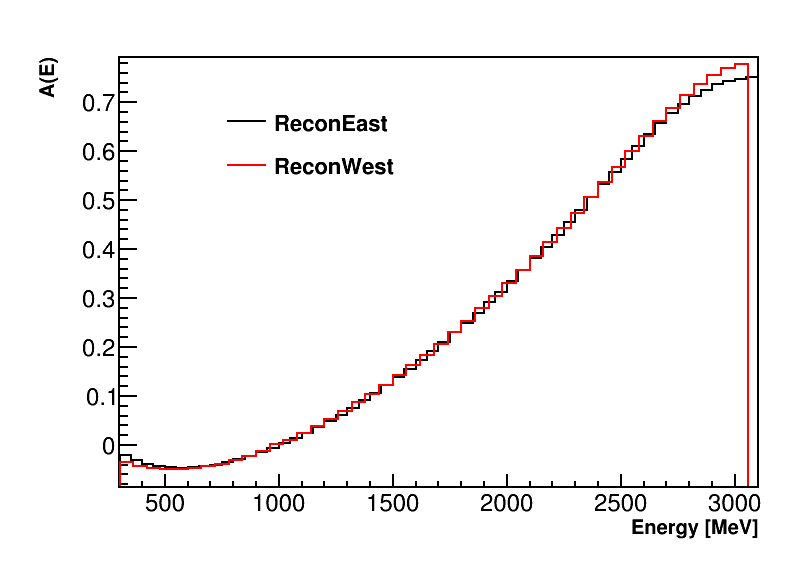
\includegraphics[width=\textwidth]{ReconEastvWest_A}
        \caption{$A(E)$}
    \end{subfigure}
    \hspace{1mm}
    \begin{subfigure}[t]{0.45\textwidth}
        \centering
        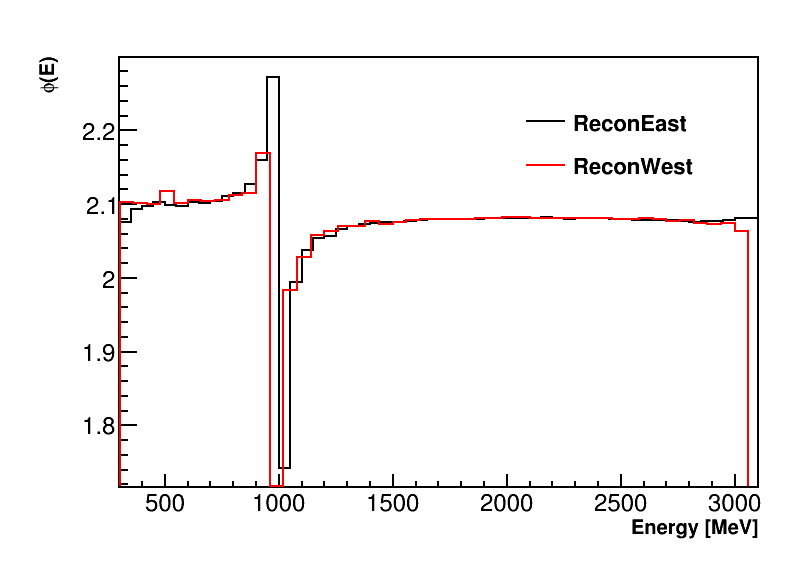
\includegraphics[width=\textwidth]{ReconEastvWest_Phi}
        \caption{$\phi(E)$}
    \end{subfigure}
\caption[]{$N$, $A$, and $\phi$ as functions of energy from energy bin fits to \RE (black) and \RW (red) data for the 9d dataset. These histograms are representative of the quantities for all datasets, though there are slight differences. The \RE energy bin fits ranged from \SIrange{300}{3100}{\MeV} in bins of \SI{50}{\MeV} for a total of 56 energy bins, while the \RW energy bin fits ranged from \SIrange{300}{3060}{\MeV} in bins of \SI{60}{\MeV} for a total of 46 energy bins, hence the different bin edges in the plot. There are some slight differences at low and high energies within the various plots, but for the most part energy bin fits to the two reconstructions behave very similarly.}
\label{fig:energyBinFits}
\end{figure}



The energy dependent terms in \equref{eq:2dfunc} were determined from energy-binned fits to the data provided by D. Sweigart for \RE and M. Sorbara for \RW reconstructions respectively, for each of the four datasets in \Rone. \figref{fig:energyBinFits} shows the respective histograms for the 9d dataset, where it can be seen that energy bin fits to the two reconstructions produce very similar histograms. The \RE energy bin fits ranged from \SIrange{300}{3100}{\MeV} in bins of \SI{50}{\MeV} for a total of 56 energy bins, while the \RW energy bin fits ranged from \SIrange{300}{3060}{\MeV} in bins of \SI{60}{\MeV} for a total of 46 energy bins. Two \texttt{TF2}s were constructed using either the \RE or \RW histograms as input. The number of Y points in the 2D functions were set as the number of energy bins in the respective histograms, and the function was defined such that the energy binned histograms would be linearly interpolated between the values at the bin centers. The number of X points in the 2D functions were set such that the function ranged from \SIrange{0}{699971.8}{ns} in steps of $149.2/2 = \SI{74.6}{ns}$ for a total of 9383 points. This `point-width' was chosen for a few reasons. The first is that the maximum number of allowed X or Y points in a \texttt{TF2} is 10000, and this point-width results in a number of points close to but not above that value. The second is that the chosen point-width was either exactly or very close to a multiple of the bin widths chosen by the analyzers. It was found that using the maximum number of points such that the point-width was \ns{70} (for a range up to \ns{700000}) resulted in aliasing frequencies appearing in the some of the FFTs of the fit residuals to the generated data. With a point-width of \ns{74.6} these aliasing frequencies disappeared entirely except in some Q-Method fits. In order to remove this issue entirely a different implementation besides that described here would be needed, with finer granularity or better interpolation. The 2D function parameters are summarized in \tabref{tab:2dfunctionParameters}.


\begin{table}[h]
\centering
\renewcommand{\arraystretch}{1.2}
\begin{tabularx}{1\linewidth}{@{\extracolsep{\fill}}lcc}
  \hline
    \multicolumn{3}{c}{\textbf{2D Function Parameters}} \\
  \hline\hline
     & \thead{\RE Input} & \thead{\RW Input} \\
  \hline
  	Energy Range (\MeV) & 300--3100 & 300--3060 \\
  	Energy Points & 56 & 46 \\ 
  	Energy Point-Width (\MeV) & 50 & 60 \\
  	Time Range (ns) & 0--699971.8 & 0--699971.8 \\
  	Time Points & 9383 & 9383 \\
  	Time Point-Width (ns) & 74.6 & 74.6 \\
  \hline
\end{tabularx}
\caption[]{Parameters used to define the \texttt{TF2}s in the Monte Carlo pseudo-data generation.}
\label{tab:2dfunctionParameters}
\end{table}



\subsection{\RE vs \RW}

The two 2D \texttt{TF2}s generate pseudo-data corresponding to either the \RE or the \RW reconstruction. In order to properly estimate correlation coefficients between reconstructions, generated hits need to be converted between the two. For this requirement, a comparison between \RE and \RW is necessary. J. LaBounty studied the different reconstructions of clusters in detail \cite{JoshEvW}. In doing so he determined that the cluster times between the two reconstructions were the same to high precision, but that there were differences in the reconstructed cluster energies. He took D. Sweigart's \RE and A. Fienberg's \RW analyses respectively, isolated clusters produced from the same waveforms, and compared the hit energies to each other. The calorimeter sum of this comparison for the 9d dataset is shown in \figref{fig:EvWenergies}. As shown most hits lie along the unit slope line. Some hits lie in different bands due to reconstruction differences in how certain hits and energies are treated\footnote{One example is that some individual crystals in some calorimeters have poor relative energy calibration between the two reconstructions.}. Taking 1D projections of this distribution, like in \figref{fig:EvWprojection}, energies can be converted between \RE and \RW by sampling those projections.


Before describing the event generation, a couple of points should be mentioned. First is that the bin width used by J. LaBounty was \SI{10}{\MeV}, discrete enough for the purposes of this Monte Carlo and also finer than the energy bin widths used in the generation of the \texttt{TF2}s. Second is that the comparison between reconstructions was built upon clusters before they had been corrected for pileup, hence the presence of counts at energies beyond the magic momentum of \SI{3.094}{\GeV} (plus the energy resolution). It is expected that this should be a fine approximation to use since pileup is a minimal effect after it has been corrected. Third is that this comparison was built upon D. Sweigart's and A. Fienberg's analyses. D. Sweigart is the only \RE analyzer, while A. Fienberg was one of several \RW analyzers. Since A. Fienberg used different clustering parameters than the rest of the \RW analyzers, (\texttt{timeCutoffLow = 2, timeCutoffHigh = 3} vs \texttt{timeCutoffLow = 3, timeCutoffHigh = 5}), the comparison isn't perfect. For the most technically correct results the \RE vs \RW comparison should be done individually for all analyzers, though the final results are not expected to change significantly.



\begin{figure}
\centering
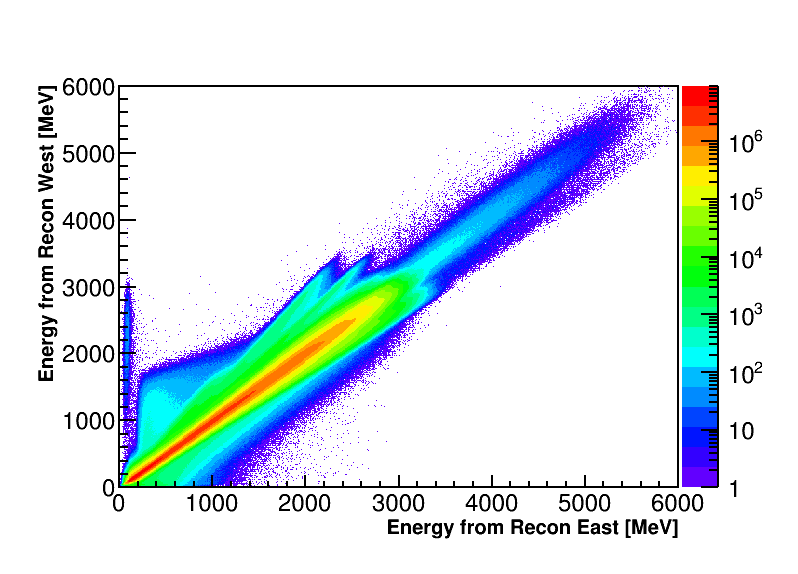
\includegraphics[width=.7\textwidth]{ReconEastvWest_Energies}
\caption{Log-scale plot of \RE energies vs \RW energies for the same produced clusters for the 9d dataset. The majority of hits form a Gaussian around the unit slope line, however there are bands of hits outside this region due to reconstruction differences in how certain hits and energies are treated. This pattern was determined to be stable throughout the fill. \RE vs \RW comparison performed by J. LaBounty \cite{JoshEvW}.}
\label{fig:EvWenergies}
\end{figure}

\begin{figure}
\centering
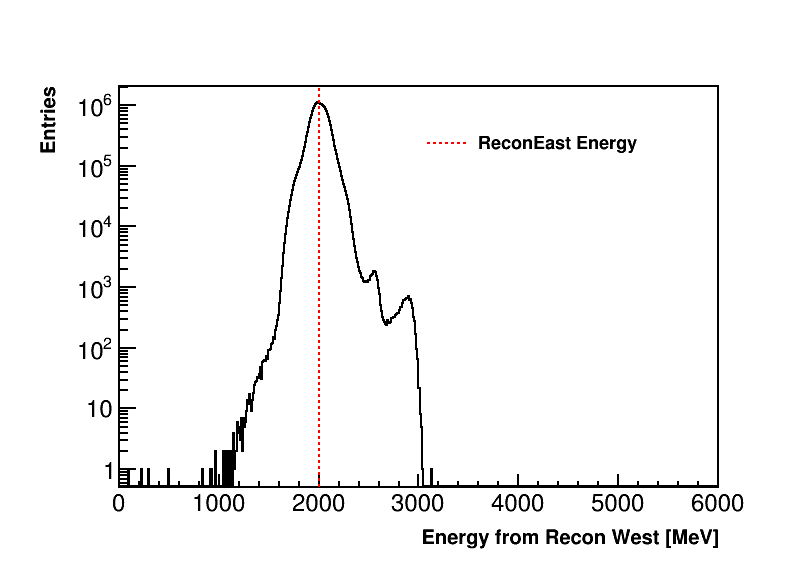
\includegraphics[width=.7\textwidth]{ReconEastvWest_Projection}
\caption{A Y-axis or \RW energy projection for a chosen \RE energy of \SI{2}{\GeV}. The plot is on a log-scale.}
\label{fig:EvWprojection}
\end{figure}




\subsection{Event Generation and Randomization}


Many samples of pseudo-data were generated via the same procedure. These samples were generated by submitting 1000 jobs each to the grid for the East-To-West and West-To-East variants\footnote{'East-To-West' means that the 2D function with input from the \RE energy binned functions was used to generate the data, and vice versa.}, for each dataset. The number of jobs which completed varied only slightly, except for the EG dataset which had less completed jobs due to timing out on the grid; see \tabref{tab:jobs}. 


\begin{table}[h]
\centering
\renewcommand{\arraystretch}{1.2}
\begin{tabularx}{0.4\linewidth}{@{\extracolsep{\fill}}lcc}
  \hline
    \multicolumn{3}{c}{\textbf{Jobs Completed}} \\
  \hline
    Dataset & East-To-West & West-To-East \\
  \hline
    60h & 1000 & 999 \\
    HK & 1000 & 999 \\
    9d & 1000 & 1000 \\
    EG & 851 & 856 \\ 
  \hline
\end{tabularx}
\caption[]{Number of jobs completed out of 1000 after submission to the grid for the East-To-West and West-To-East variants. When calculating the statistical errors on the calculated correlation coefficients, the smaller of the two numbers corresponding to the larger error is used.}
\label{tab:jobs}
\end{table}


The number of hits per dataset was determined empirically such that the error on the fitted \R values were comparable to the \Rone results shown in \tabref{tab:analysisRValues}. The approximate level of statistics for the 60h, HK, 9d, and EG datasets are given by the counts \{5.04e9, 7.01e9, 1.08e10, 2.21e10\} respectively. Note that these numbers depend on the energy and time ranges of the \texttt{TF2}s and hence do not correspond directly to the real dataset statistics; what was important and thus replicated was the number of hits which ended up in the wiggle plot within the fit ranges. The errors on the fitted \R values were always within \SIrange{10}{20}{ppb} of the actual real data analysis values (and many times within a few ppb).

Note that in the event generation no time-randomization was included, as is done by the analyzers in order to remove effects of the fast rotation. It is expected that in the Monte Carlo with no fast rotation effect, with enough random seeds, the mean fitted \R value is equivalent to the non-time-randomized \R value. While the spread in the \R values will be slightly less without the time-randomization, this is expected to negligibly affect the final correlation coefficients. This effect could in the future be included at the expense of more processing time, where it is expected that the event generation would take significantly longer.

The procedure for the event generation was as follows:
\begin{enumerate}
	\item{A number of hits per sample and per dataset was determined via \texttt{PoissonD()} method calls on the static number of statistics per dataset such that each sample had a very slightly different amount of statistics.} 
	\item{For each hit or entry, \texttt{TF2->GetRandom2()} is called on one of the two 2D input functions, with either \RE or \RW input, to generate a time and energy for a hit.}
	\item{For either variant, East-To-West or West-To-East, the corresponding \RW or \RE energy was determined by randomly sampling the corresponding energy projection as determined from J. LaBounty's studies. This projection was sampled via \texttt{TH1->GetRandom()} method calls. The first generated energy, designated either as \RE or \RW, was also designated as the Q-Method energy.}
	\item{The generated time-energy pairs were then used to fill histograms defined by the analyzer parameters given in \tabref{tab:analyzerParameters}, with the corresponding weights set according to the specific analysis types. In the A-Method histograms, the asymmetry weights were determined from a linear interpolation of the asymmetry energy binned histogram, while in the Q-Method histograms the energies themselves were used as the weights.}
	\item{The R-Method has intrinsic randomization in how the counts get put into the four ratio histograms, and so ratio histograms were produced for 100 different random seeds. The randomization of counts was performed via \texttt{GetUniform()} method calls in order to properly distribute the data.}
\end{enumerate}


In all instances of the randomization, including the randomization on the number of events, sampling the \texttt{TF2}s, sampling the \RE vs \RW energy projections, and the ratio randomization, the \ROOT \texttt{TRandomMixMax} class is used. The standard \texttt{TRandom3} class was initially used and found to be inadequate for this high precision statistical study. \texttt{TRandomMixMax} has the advantage of producing better random numbers with high periodicity, and also being fast enough to produce the high statistics in a reasonable time frame\footnote{This generator is the default used in Geant4.}\cite{TRandom}.



\subsection{Fitting the Pseudo-Data}


Once the pseudo-data had been generated, the data was fit either with a simple five parameter function in the TAQ-Methods,
\begin{align}
    N(t) = N_{0} \cdot e^{-t/\tau_{\mu}} \cdot (1 + A \cos{(\omega_{a}t + \phi})),
\label{eq:fiveParFit}
\end{align}
or a simple three parameter function in the case of the R-Method,
\begin{align}
    R(t) =A \cos{(\omega_{a}t + \phi}),
\label{eq:ratioFit}
\end{align}
with fit ranges defined by the associated parameters in \tabref{tab:analyzerParameters}. In both cases the energy dependent pieces from \equref{eq:2dfunc} are gone, and the fitted constants in general converge to their average integrated values. \figref{fig:sampleFits} shows examples of fits to the four different methods, for the same generated sample. In general the fit parameters are very similar to one another between the different methods, however due to the different analyzer specific parameters like energy threshold, the fit parameters can be slightly, but significantly, different. \figref{fig:FFTs} shows the FFTs of the fit residuals from \figref{fig:sampleFits}. What sometimes occurred, though isn't shown here, is that aliasing peaks can appear at beat frequencies with \wa, due to differences in the point-width frequency of the input 2D function and the bin width of the histogram. 

Once all samples and seeds were fitted, the fit parameters were stored into \ROOT trees such that the parameters for the different methods and samples could be compared. Similarly, measures of the goodness-of-fit were also stored, in order to verify that the pseudo-data was being fit correctly. P value distributions for the four methods for one set of samples is shown in \figref{fig:pValues}. As shown the distributions are flat for the T and A-Methods, and are not flat for the R and Q-Methods. The Q-Method is understood to be non-flat due to the difference in bin width and point-width mentioned previously, while the origin of the non-flatness of the R-Method is unkwown at this time\footnote{It may be that the random generator class \texttt{TRandomMixMax} is insufficient for the ratio method randomization, which performs many more randomization calls than the other methods.}. \figref{fig:pulls} show the pulls on \R for the different samples in the same set of fitted samples. The distributions in general are very close to unit-Gaussians, with some slight deviations in the R and Q-Method cases leading to slight pulls on \R. This should have a very minimal effect on the calculated correlation coefficients, but it should be kept in mind.


\begin{figure}
\centering
    \begin{subfigure}[t]{0.45\textwidth}
        \centering
        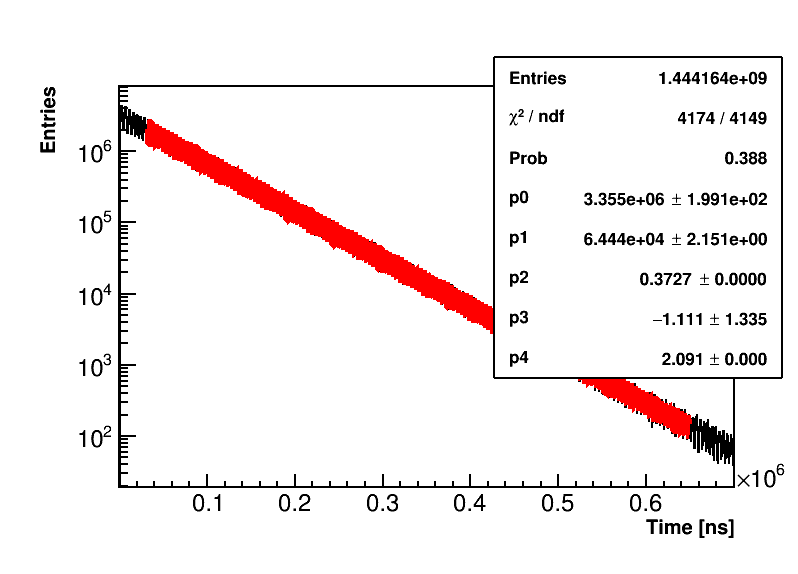
\includegraphics[width=\textwidth]{Example_TMethod_Fit}
        \caption{T-Method}
    \end{subfigure}
    \hspace{1mm}
    \begin{subfigure}[t]{0.45\textwidth}
        \centering
        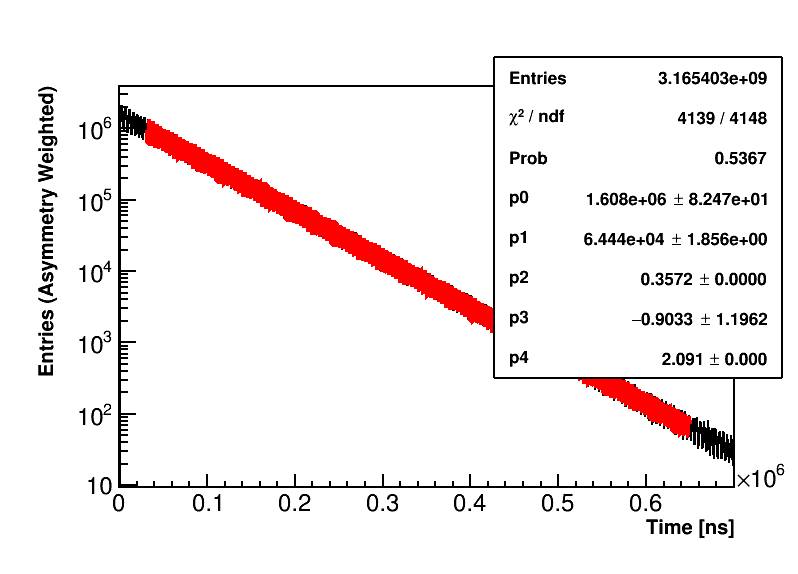
\includegraphics[width=\textwidth]{Example_AMethod_Fit}
        \caption{A-Method}
    \end{subfigure}% %you need this % here to add spacing between subfigures

    \begin{subfigure}[t]{0.45\textwidth}
        \centering
        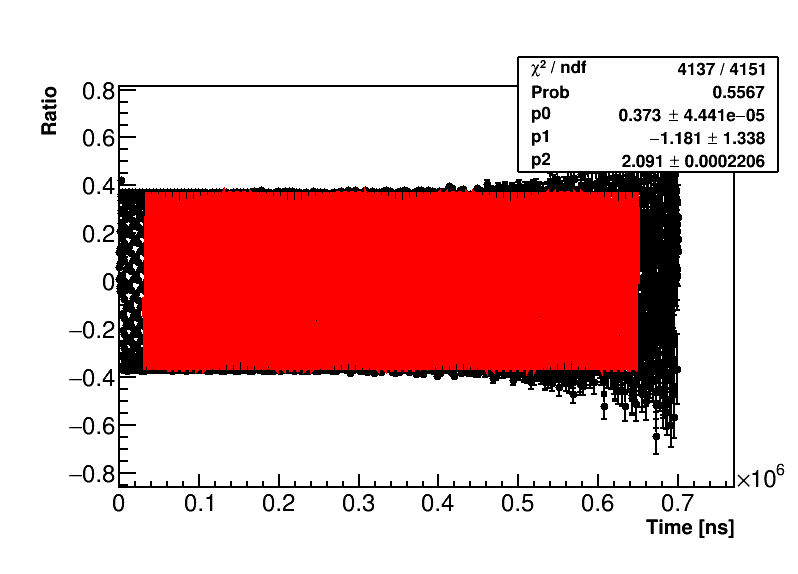
\includegraphics[width=\textwidth]{Example_RMethod_Fit}
        \caption{R-Method}
    \end{subfigure}
    \hspace{1mm}
    \begin{subfigure}[t]{0.45\textwidth}
        \centering
        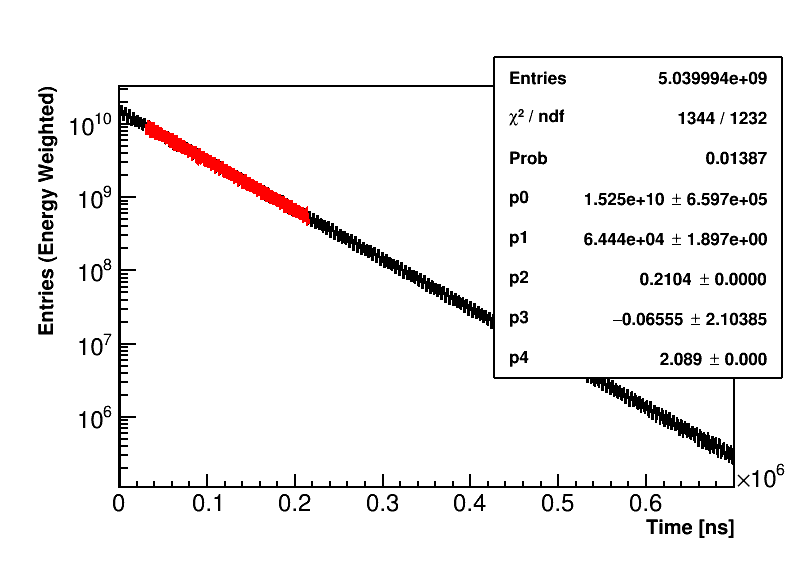
\includegraphics[width=\textwidth]{Example_QMethod_Fit}
        \caption{Q-Method}
    \end{subfigure}
\caption[]{TARQ-Method fits to a sample generated from the 60h East-To-West Monte Carlo data.}
\label{fig:sampleFits}
\end{figure}
%-T method was from Aaron, A method from David, R method from me, and Q from Tim


\begin{figure}
\centering
    \begin{subfigure}[t]{0.45\textwidth}
        \centering
        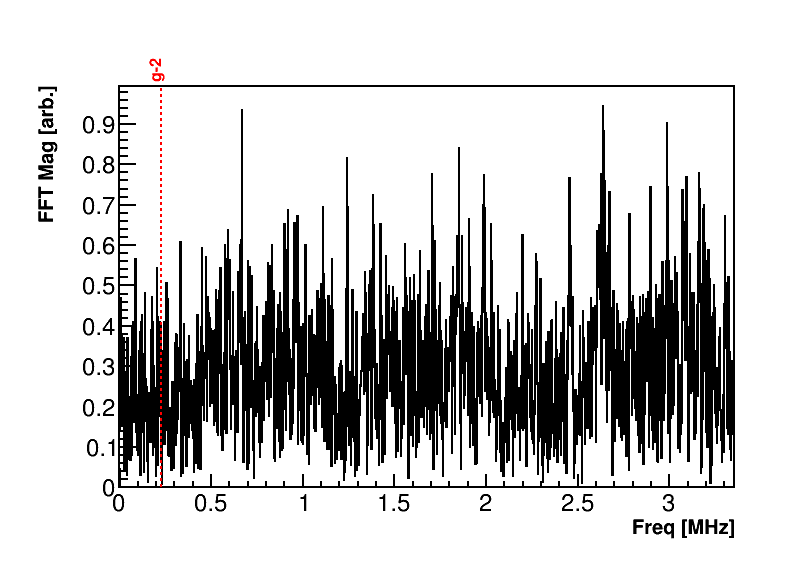
\includegraphics[width=\textwidth]{FFT_TMethod}
        \caption{T-Method}
    \end{subfigure}
    \hspace{1mm}
    \begin{subfigure}[t]{0.45\textwidth}
        \centering
        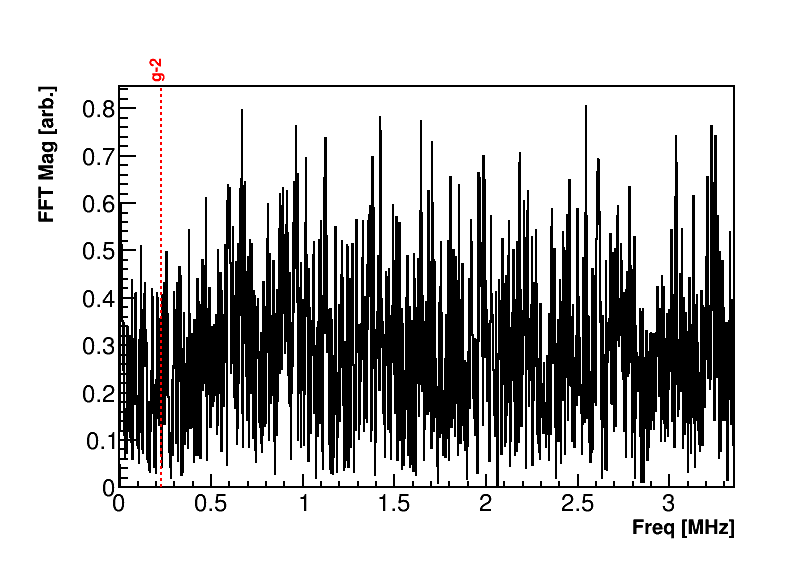
\includegraphics[width=\textwidth]{FFT_AMethod}
        \caption{A-Method}
    \end{subfigure}% %you need this % here to add spacing between subfigures

    \begin{subfigure}[t]{0.45\textwidth}
        \centering
        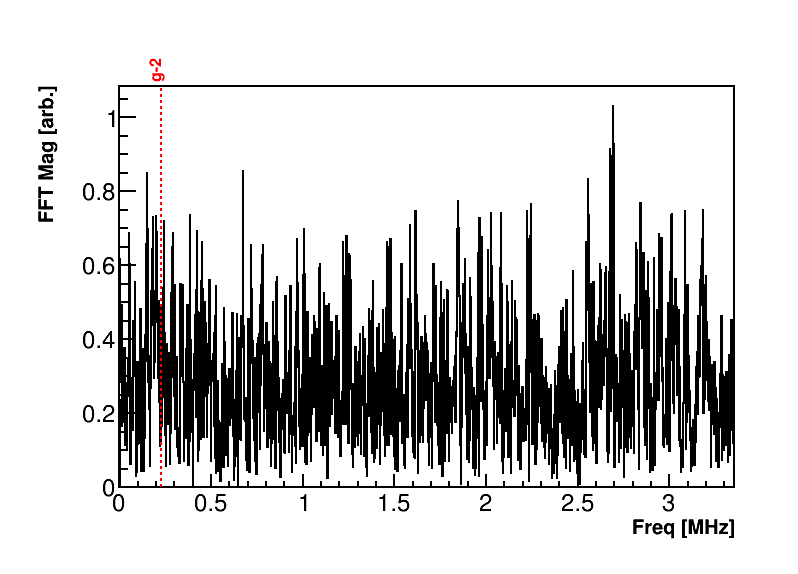
\includegraphics[width=\textwidth]{FFT_RMethod}
        \caption{R-Method}
    \end{subfigure}
    \hspace{1mm}
    \begin{subfigure}[t]{0.45\textwidth}
        \centering
        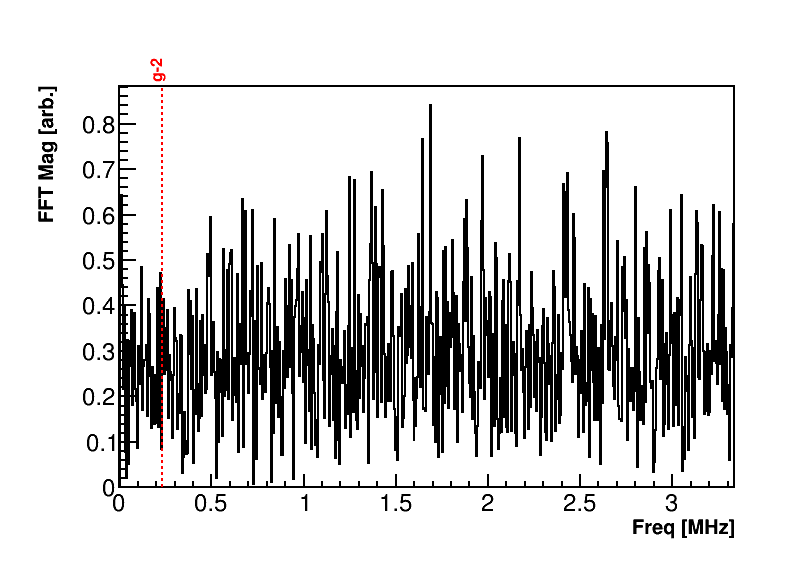
\includegraphics[width=\textwidth]{FFT_QMethod}
        \caption{Q-Method}
    \end{subfigure}
\caption[]{FFTs of the fit residals for those fits shown in \figref{fig:sampleFits}. No peaks rise above the noise, though in some Q-Method fits an aliasing frequency between \gmtwo and the point-width of the generating function can be seen.}
\label{fig:FFTs}
\end{figure}


\begin{figure}
\centering
    \begin{subfigure}[t]{0.45\textwidth}
        \centering
        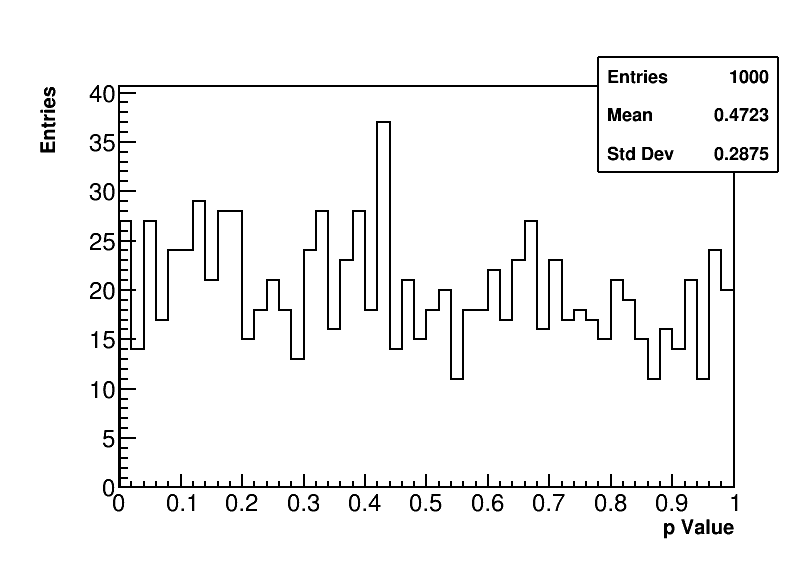
\includegraphics[width=\textwidth]{PValues_TMethod}
        \caption{T-Method}
    \end{subfigure}
    \hspace{1mm}
    \begin{subfigure}[t]{0.45\textwidth}
        \centering
        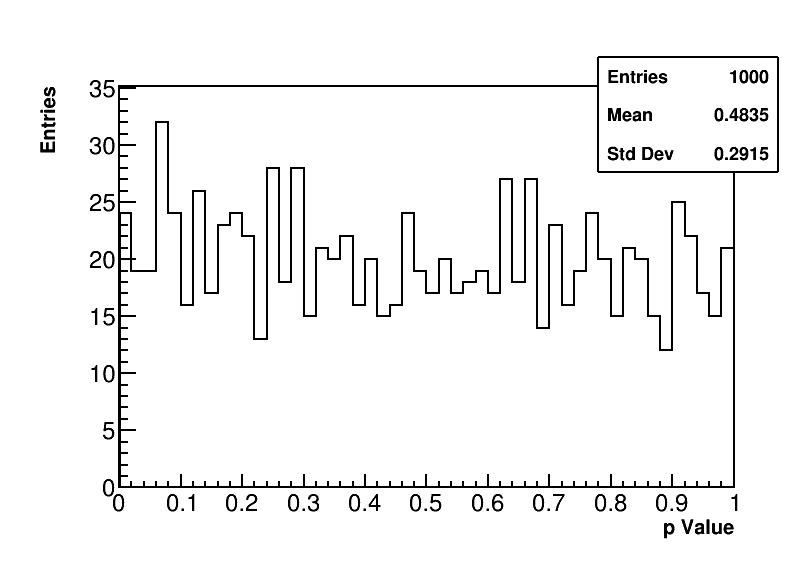
\includegraphics[width=\textwidth]{PValues_AMethod}
        \caption{A-Method}
    \end{subfigure}% %you need this % here to add spacing between subfigures

    \begin{subfigure}[t]{0.45\textwidth}
        \centering
        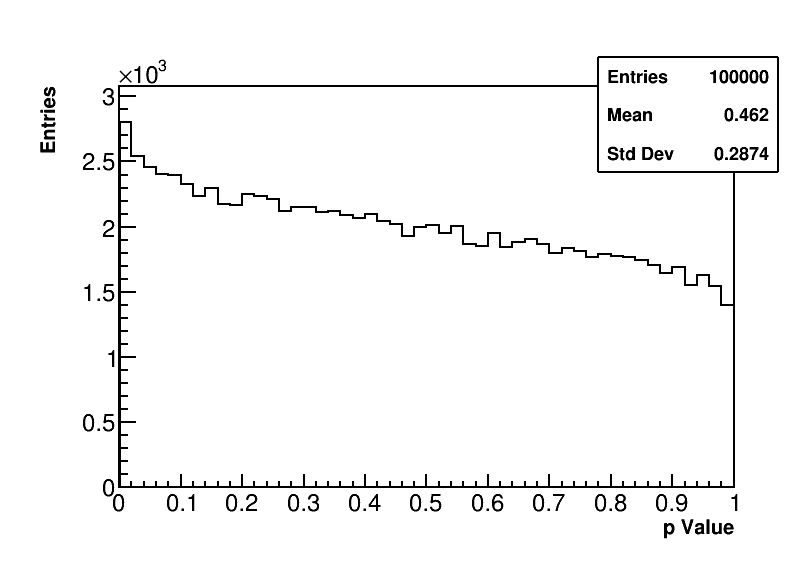
\includegraphics[width=\textwidth]{PValues_RMethod}
        \caption{R-Method}
    \end{subfigure}
    \hspace{1mm}
    \begin{subfigure}[t]{0.45\textwidth}
        \centering
        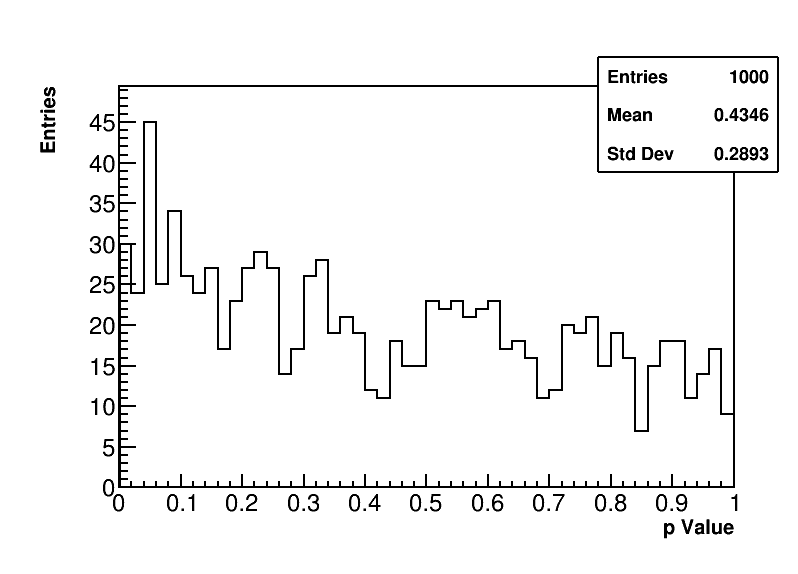
\includegraphics[width=\textwidth]{PValues_QMethod}
        \caption{Q-Method}
    \end{subfigure}
\caption[]{P value distributions for fits to 1000 samples, for the 60h East-To-West Monte Carlo pseudo-data. The T and A-Method p values are flat, while the R and Q-Method p values are not. In the case of the Q-Method, the non-flat shape can be attributed to the difference in bin width and 2D function point-width. The origin of the non-flat shape for the R-Method is unknown at this time.}
\label{fig:pValues}
\end{figure}


\begin{figure}
\centering
    \begin{subfigure}[t]{0.45\textwidth}
        \centering
        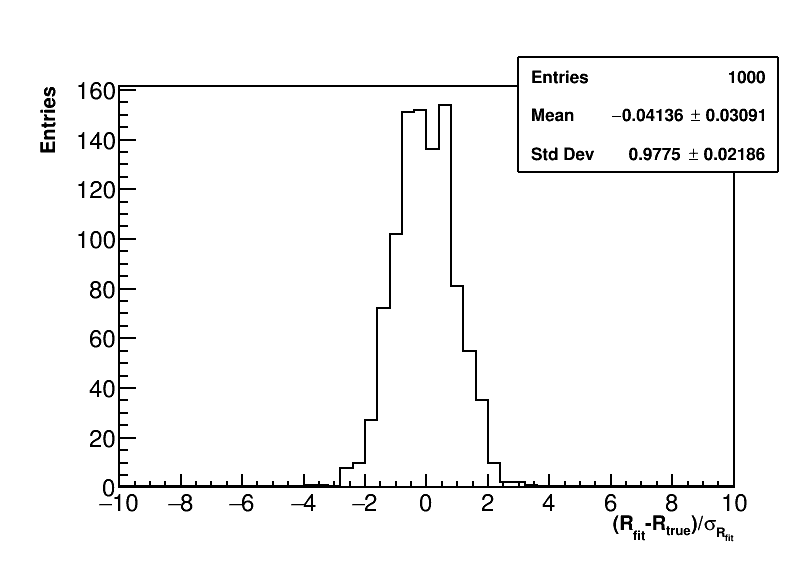
\includegraphics[width=\textwidth]{Rpull_TMethod}
        \caption{T-Method}
    \end{subfigure}
    \hspace{1mm}
    \begin{subfigure}[t]{0.45\textwidth}
        \centering
        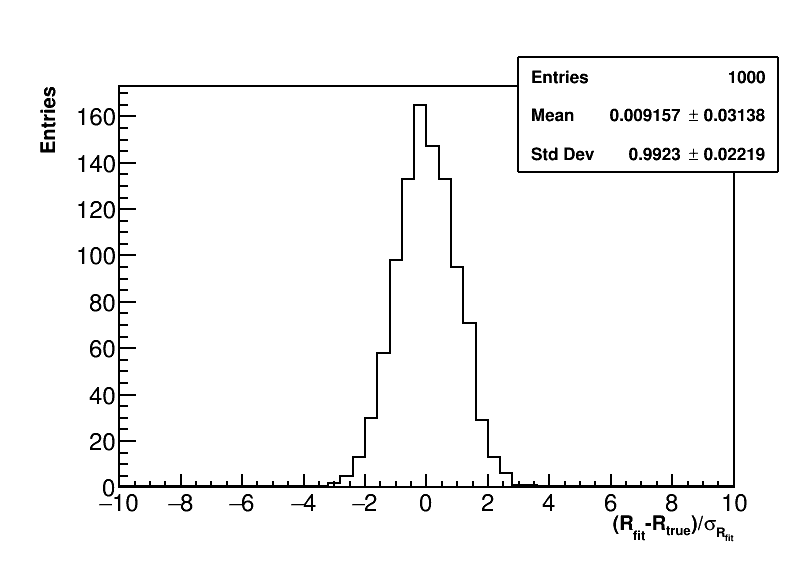
\includegraphics[width=\textwidth]{Rpull_AMethod}
        \caption{A-Method}
    \end{subfigure}% %you need this % here to add spacing between subfigures

    \begin{subfigure}[t]{0.45\textwidth}
        \centering
        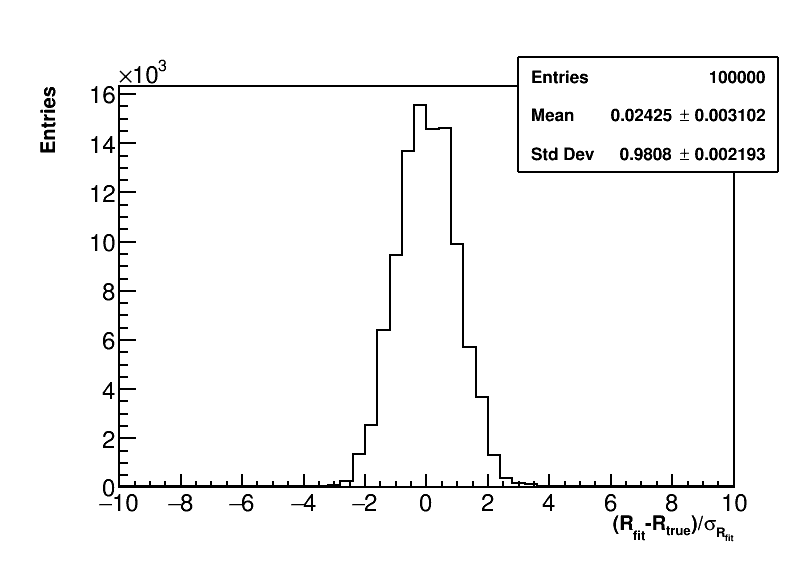
\includegraphics[width=\textwidth]{Rpull_RMethod}
        \caption{R-Method}
    \end{subfigure}
    \hspace{1mm}
    \begin{subfigure}[t]{0.45\textwidth}
        \centering
        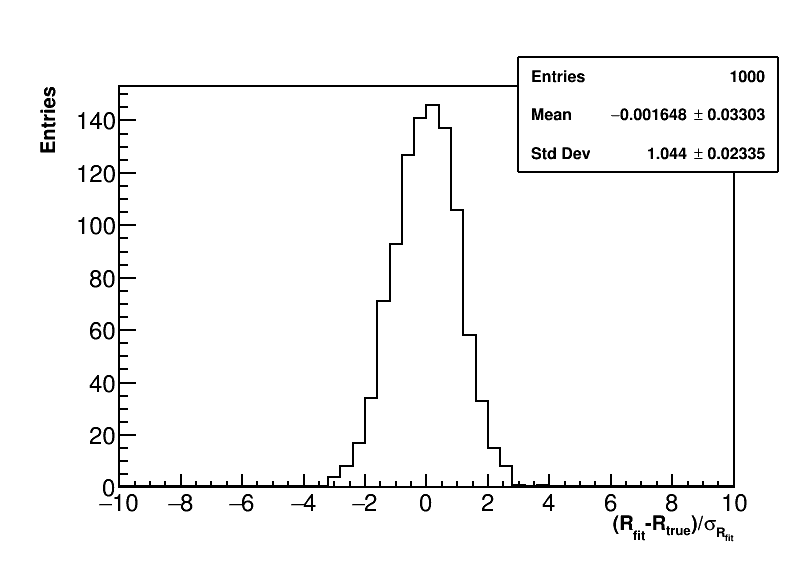
\includegraphics[width=\textwidth]{Rpull_QMethod}
        \caption{Q-Method}
    \end{subfigure}
\caption[]{Pull distributions for fits to 1000 samples, for the 60h East-To-West Monte Carlo pseudo-data. The various distributions are close to unit-Gaussians, with differences in some R and Q-Method cases which is attributed to imperfect data-generation.}
\label{fig:pulls}
\end{figure}


\clearpage
\subsection{Calculating the Correlations and Errors}


Once the generated pseudo-data was fitted, the \R values and other parameters were plotted against one another for different analyses and methods to determine the correlation coefficients. An example of such a scatter plot is shown in \figref{fig:scatterPlot}. The final correlation coefficients are calculated as the average of the correlation coefficients produced with the East-To-West and West-To-East variants. The systematic errors on the coefficients are determined as the difference between the average correlation coefficients and either of the two variants. The statistical error on the determined correlation coefficients is dependent on the number of points or samples used to calculate the coefficients as well as the coefficients themselves. These statistical errors are calculated via the Fisher-$z$ transform of the correlation coefficients $r$,
\begin{align}
    z = \tanh^{-1}r,
\end{align}
where the variance on $z$ goes as
\begin{align}
    V(z) = \frac{1}{n-3},
\end{align}
and $n$ is the number of samples. By converting the correlation coefficients $r$ to $z$, finding the upper and lower ranges when adding or subtracting the square root of the variance, and then converting back to $r$, the statistical errors are determined. This is described more fully in Section~9.5 of G. Cowan's \textit{Statistical Data Analysis} \cite{Cowan}. The positive and negative statistical errors as a function of the correlation for 851 samples is shown in \figref{fig:statError}. As shown the statistical error decreases as the correlation increases. To quote a single statistical error for each correlation coefficient, the average of the positive and negative errors was taken. As shown the error is $\mathcal{O}(10^{-2} - 10^{-4})$ depending on the correlation coefficient. The statistical errors are sometimes comparable to the systematic errors, and sometimes much less. By definition the systematic error will include it's own statistical error since the two variants come from different grid job submissions, however the extra error is simply conservatively included in the systematic number. The total error is then the quadrature sum of the statistical and systematic errors as usual.




\begin{figure}
\centering
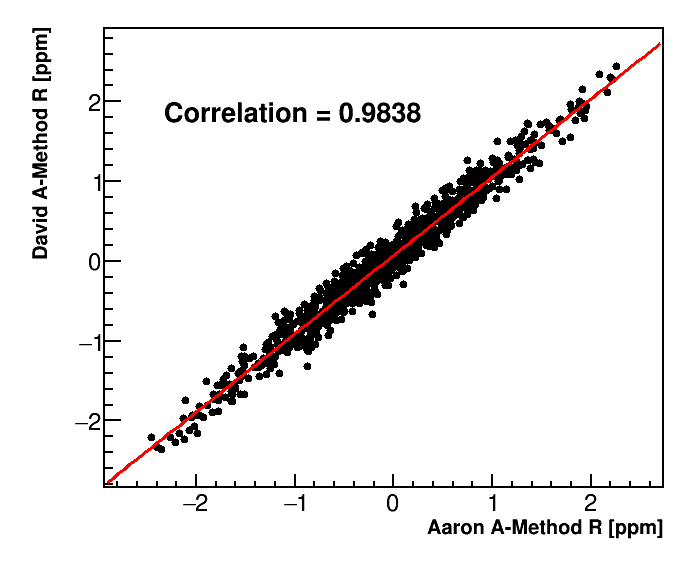
\includegraphics[width=0.5\textwidth]{ScatterPlot}
\caption{Scatter plot between \R values for two different analyses, from jobs submitted for the 9d dataset East-To-West variant. The correlation coefficient between these two analyses is determined from this scatter plot, and the red line simply guides the eye.}
\label{fig:scatterPlot}
\end{figure}



\begin{figure}
\centering
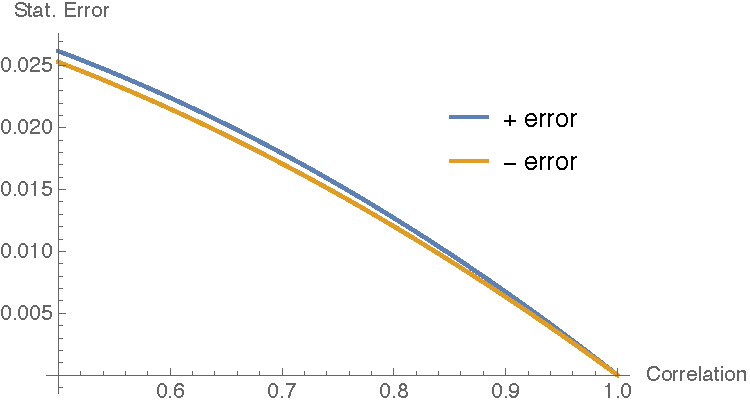
\includegraphics[width=0.5\textwidth]{StatisticalError}
\caption{Positive and negative statistical errors on the correlation coefficient as a function of the correlation, for 851 samples.}
\label{fig:statError}
\end{figure}


